% This is LLNCS.DEM the demonstration file of
% the LaTeX macro package from Springer-Verlag
% for Lecture Notes in Computer Science,
% version 2.4 for LaTeX2e as of 16. April 2010
%
\documentclass[spanish]{llncs}
%
% \usepackage{standalone}
\usepackage{pdfpages}
\usepackage{graphicx}
\usepackage[spanish]{babel}
\usepackage[utf8]{inputenc}
\usepackage{makeidx}  % allows for indexgeneration
\usepackage{url}

\setlength{\parskip}{\smallskipamount}
\setlength{\parindent}{0pt}
\usepackage{amssymb}
\usepackage{float}
%
\begin{document}
%

\mainmatter              % start of the contributions
%
\title{Análisis de la herramienta TLA+ Proof System}
%
%
\author{Pablo Celayes, Giovanni Rescia, Ariel Wolfmann}

%
\institute{Facultad de Matemática, Astronomía y Física\\
Universidad Nacional de Córdoba}

\maketitle              % typeset the title of the contribution

\begin{abstract}
Analizamos el lenguaje de especificación de alto nivel TLA+ y sus herramientas.
Nos enfocamos particularmente en \textit{TLA+ Proof System}, un entorno de verificación automática de pruebas formales.
Estudiamos su contexto de creación, sus características y aplicaciones en la industria.
Comparamos el lenguaje y sus herramientas con otros similares e ilustramos su forma de uso con un ejemplo algorítmico sencillo.
\end{abstract}
%

\section{Contexto de creación de la herramienta}

 En 1977, Amir Pnueli introdujo el uso de lógica temporal para describir el comportamiento de un sistema, lo cual en principio podía hacerse en una sola fórmula pero no resultaba así en la práctica. La lógica temporal de Pnueli era ideal para describir ciertas propiedades, pero poco adecuada para muchas otras, por lo que normalmente se la combinaba con maneras más tradicionales de describir sistemas. \cite{pnueli} A fines de los 80's Leslie Lamport inventó el lenguaje TLA (Temporal Logic of Actions), una variante simple de la lógica temporal de Pnueli que facilita la descripción de un sistema completo en una sola fórmula usando mayormente Matemática ordinaria (no temporal) y reservando la lógica temporal sólo para aquellas propiedades en las que realmente es buena. \cite{specsys}
 
 En 2001, Lamport comenzó a trabajar en el centro \textit{Microsoft Research} de Mountain View, Estados Unidos. De esta etapa surge el proyecto TLA+ Proof System (TLAPS) que actualmente se desarrolla como parte del proyecto \textit{Tools for Proofs} en el centro conjunto de investigación \textit{Microsoft Research - INRIA} de Palaiseau, Francia. 
 El proyecto continúa en desarrollo activo y cuenta con una activa lista de mail y un sistema público de seguimiento de \textit{bugs}.

% Comentar repercusiones, cómo es que termina en Microsoft y cómo se relacione esto con la evolución del Toolbox y sus aplicaciones en la industria.

% Distinguir TLA y TLA+

\section{Objetivo de la herramienta}

TLAPS es una herramienta que verifica mecánicamente la correctitud de pruebas escritas en TLA+.
Éste es un lenguaje de especificación de propósito general, orientado a sistemas concurrentes y distribuidos\cite{highlevel}.
En general, una prueba de TLA+ es una colección de sentencias estructuradas jerárquicamente,
donde cada sentencia tiene una afirmación, injustificada o justificada por una colección de hechos citados.
El propósito de TLAPS es verificar las pruebas de teoremas propuestas por el usuario, es decir,
que la jerarquía de las sentencias de hecho establecen la veracidad del teorema si las afirmaciones fueran ciertas,
y luego verificar que la afirmación de cada sentencia justificada es implicada por los hechos citados\cite{tlaps}.
Si un teorema de TLA+ tiene una prueba con todas sus afirmaciones justificadas, entonces, como resultado
de comprobar la prueba, TLAPS verifica que el teorema es cierto.

\section{Descripción de la herramienta del lado del usuario}
TLA+ es un lenguaje de alto nivel para la descripción de sistemas, especialmente sistemas concurrentes asíncronos y distribuidos. 
Fue diseñado para ser simple, muy expresivo, y permitir una formalización directa del razonamiento de aserciones tradicional.
Se basa en la idea de que la mejor manera de describir formalmente es con matemática simple, y que un lenguaje de especificación debe contener lo menos posible más allá de lo que se necesita para escribir matemática simple con precisión. Para cumplir con el objetivo de formalizar el razonamiento de aserciones, TLA+ está basado en TLA (\textit{Temporal Logic of Actions}), una variante simple de la lógica temporal lineal.

% itemizar esto, mencionar toolbox
TLA+ posee una interfaz gráfica (\textbf{Toolbox}) desde la cual trabajar con las siguientes herramientas de modo sencillo e integrado:

  \begin{itemize}
    \item \textbf{PlusCal} se usa como lenguaje intermedio para realizar la especificaciones. Es un lenguaje algorítmico que a primera vista parece un lenguaje de programación imperativo pequeño, pero es bastante más expresivo. Un algoritmo PlusCal se traduce (compila) en una especificación TLA+, la cual puede ser chequeada con las herramientas de TLA+.
	  Fue diseñado para combinar la sencillez del pseudocódigo con la expresividad de un lenguaje formalmente definido y verificable, permitiendo que personas sin mucho conocimiento en matemática formal puedan escribir especificaciones de forma cómoda y luego traducirlas a TLA+ usando la herramienta de traducción provista.
    \item En un \textbf{Modelo Standard}, un sistema abstracto se describe como un conjunto de comportamientos, cada uno representando una posible ejecución del sistema, donde un comportamiento es una secuencia de estados y un estado es una asignación de valores a las variables.
	  En este modelo, un evento, también llamado un paso, es la transición de un estado a otro en un comportamiento.
    \item El chequeador de modelos \textbf{TLC} construye un modelo de estado finito de las especificaciones TLA+ para el control de las propiedades de invariancia.
	  Genera un conjunto de estados iniciales que satisfacen la especificación y a continuación realiza una búsqueda en amplitud (Breadth-First Search) sobre todas las transiciones de estado definidas. 
	  La ejecución se detiene cuando todas las transiciones de estado conducen a estados conocidos. Si TLC descubre un estado que viola un invariante del sistema, se detiene y ofrece una traza infractora. En caso de que haya alcanzado un estado que no tenga posibles acciones habilitadas, reporta un mensaje de error explicitando el posible \textit{deadlock} (opcional).
	  Dada la alta expresividad de TLA+, ningún chequeador de modelos puede manejar todas sus especificaciones. TLC maneja un subconjunto de TLA+ que intenta incluir la mayoría de las especificaciones algorítmicas y propiedades de corrección, así como todas las especificaciones de diseño de protocolos y sistemas.
    \item \textbf{TLA+ Proof System} es una plataforma que extiende a TLA+ para el desarrollo y verificación mecánica de demostraciones. 
	  El lenguaje de pruebas de TLA+ es declarativo y requiere cierto conocimiento previo de matemática elemental. Soporta desarrollo incremental y verifica la estructura jerárquica de la demostracion. Una demostración se traduce en un conjunto de pruebas independientes, que luego se intentan chequear usando una colección de verificadores que incluye demostradores de teoremas, asistentes de pruebas, chequeadores de satisfacibilidad y procedimientos de decisión.
	  TLAPS maneja casi toda la parte no temporal de TLA+ y el razonamiento temporal necesario para probar propiedades de seguridad (\textit{safety}) estándar (como invariantes y simulación de transiciones), pero no para propiedades de vitalidad (\textit{liveness}).
	  Desarrollar demostraciones es complejo y propenso a errores, por lo que previo a verificar la correctitud de una especificación
	  se recomienda chequear instancias finitas con TLC para detectar errores rápidamente. 
	  Una vez que TLC no encuentra errores, se puede intentar probar la correctitud de la demostración.
	  De aquí en adelante nos enfocaremos en esta última herramienta. 
  \end{itemize}

\section{Aspectos técnicos de la herramienta}
La arquitectura general de TLAPS (Fig. 1) se divide en: el administrador de pruebas de LTA (\textit{LTAPM}) y tres \textit{backends} que éste invoca: Isabelle, Zenon y SMT (Satisfiability Modulo Theories).

\begin{figure}
  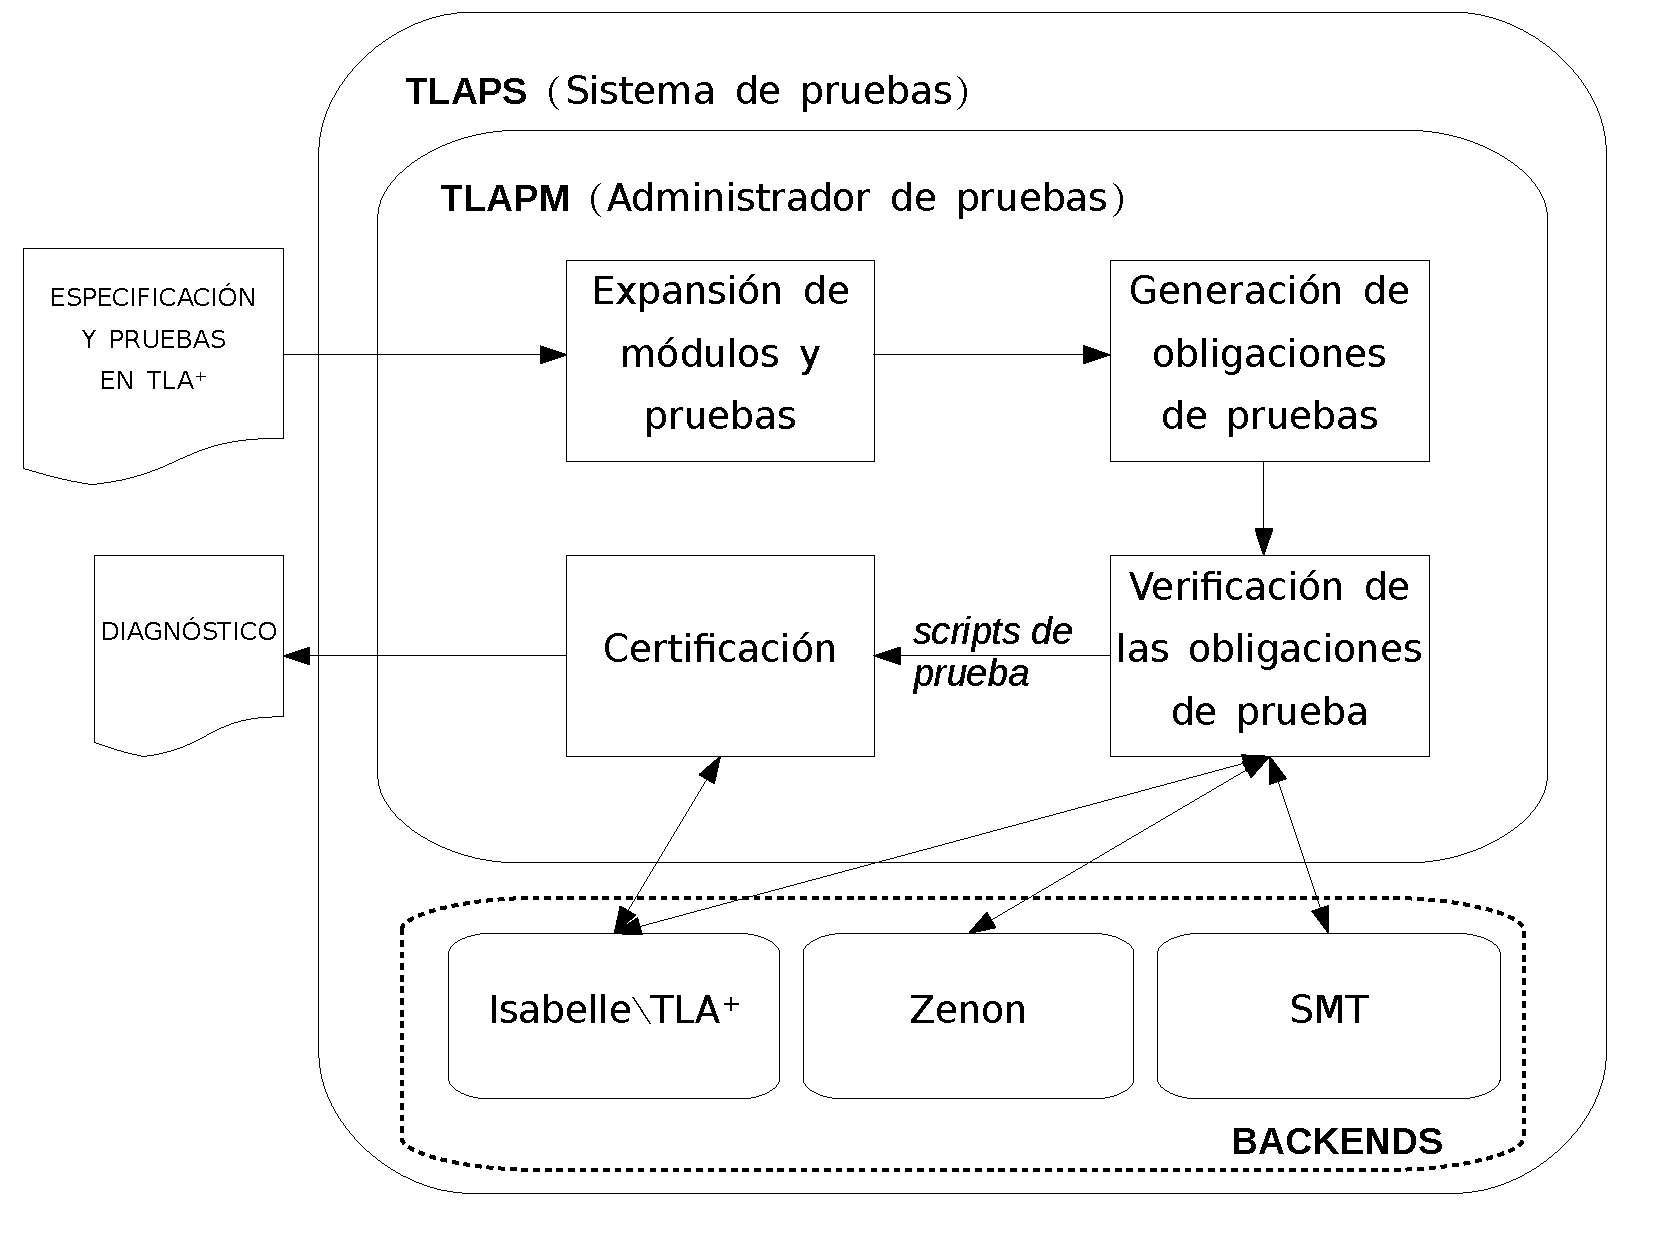
\includegraphics[scale=0.4]{esquema-informe-ingsoft2}
  \caption{Arquitectura general del entorno de pruebas TLAPS}
\end{figure}

  \textbf{LTAPM}: Una especificación en TLA+ consiste de un módulo raíz que puede (transitivamente), importar otros módulos por extensión e instanciación con
  sus respectivos parámetros. Cada módulo consiste en: parámetros (variables, o estados, y constantes sin interpretar), definiciones, teoremas, que pueden tener su prueba.
  
  Un parámetro de un módulo puede ser una variable (estado), o una constante; en las fórmulas de TLA+ no se hace referencia explícita a las variables, en cambio, se usan dos copias de una variable \textit{v}: \textit{v} y \textit{v'}, que hacen referencia a un valor antes, y después de la transición. 
  TLAPS se ejecuta invocando a TLAPM en el módulo raíz e indicando qué pruebas chequear. 
  Luego TLAPM, genera \textit{obligaciones de prueba} para cada prueba terminal, o sea, las cosas que se tienen que corroborar, para probar la correctitud del teorema. Una vez generadas, invoca a los backends para que las verifiquen.
  Si éstos no pueden encontrar una prueba en un límite razonable de tiempo, el sistema informará cuál obligación es la que falló, junto con su contexto (falló, cancelada por el usuario, omitida) y objetivo de la prueba.
  El usuario debe entonces determinar la causa de la falla (debido a que depende de hechos o definiciones ocultas, o si el objetivo es demasiado complejo y necesita ser refinado con otro nivel de prueba). Esto indica que pueden haber obligaciones que son ciertas, y que por una cuestión de \textit{timeout},
  el backend las verifica como falsas.
  Si un backend puede verificar una obligación de prueba, genera una traza de la prueba realizada, llamada \textit{certificación de prueba}.
  Finalmente, luego de certificar todas las obligaciones de prueba posibles generadas por las pruebas
  terminales, se procede a certificar el teorema en sí, en un proceso de dos pasos: primero LTAPM genera la estructura de un lema (y sus pruebas en Isabelle/TLA+) que establece simplemente que la colección de
  obligaciones de pruebas terminales implican el teorema. Luego, LTAPM genera una prueba del teorema usando la estructura del lema y las obligaciones ya certificadas. Si Isabelle acepta la prueba, estamos seguros de que la versión traducida del teorema es verdadera en Isabelle/TLA+.\cite{verifyingsafety}

  Los backends que el TLAPM invoca son: \textbf{Isabelle} es un demostrador de teoremas genérico, diseñado para hacer razonamiento interactivo en una variedad de teorías formales. Provee un lenguaje para describir las lógicas-objeto y para probar sus teoremas. Es invocado cuando la prueba en Zenon falla\cite{verifyingsafety}.
  \textbf{Zenon}, es un demostrador de teoremas automático para lógica clásica de primer orden (con igualdad), 
  basado en el método \textit{tableau}. Inicialmente diseñado para generar pruebas chequeables en el demostrador de teoremas Coq. Ahora extendido para generar scripts de pruebas chequeables en Isabelle. Uno de sus objetivos de diseño es resolver problemas simples de manera rápida\cite{zenon}. \textbf{SMT} es el backend invocado por defecto. Es particularmente bueno en problemas difíciles que involucran aritmética, funciones sin interpretar y cuantificadores.\cite{formaltech}

\section{Casos de aplicación de la herramienta}
Mencionamos a continuación algunos ejemplos de aplicación de las herramientas analizadas.
Fue difícil encontrar un ejemplo de la industria donde se use el \textit{Proof System}, el enfoque más habitual resulta ser usar PlusCal y TLA+ para especificar el diseño del sistema y las propiedades deseadas (generalmente de \textit{safety} o \textit{liveness}), y luego usar el \textit{model checker} TLC para intentar asegurar que no existan trazas de ejecución que violen las propiedades esperadas.

\textbf{Amazon}: \textit{Amazon Web Services} utiliza TLA+ desde 2011. Haciendo \textit{model checking} sobre especificaciones en TLA+ se han descubierto bugs
en DynamoDB, S3, EBS, y en un \textit{lock manager} interno distribuído.
Muchos de los bugs encontrados eran críticos pero muy sutiles, requiriendo algunos trazas de hasta 35 pasos para ser detectados.
También se ha usado model checking para verificar optimizaciones agresivas.
Además, las especificaciones TLA+ han resultado valiosas como documentación y ayudas de diseño.
Inicialmente se intentó trabajar con Alloy, pero no resulto suficientemente expresivo.
Se ha encontrado además que TLA+ es también muy práctico para modelado de datos y diseño de propiedades de \textit{schemas}. \cite{amazon}

\textbf{XBOX 360}: Microsoft usó TLA+ para encontrar y resolver un \textit{bug} en el sistema de memoria de la consola \textit{XBOX 360}.
De no haberse descubierto, cada \textit{XBOX 360} se habría colgado pasadas las 4 horas de uso.
\cite{xbox360}

\textbf{Byzantine Paxos}: Leslie Lamport usó el TLAPS para derivar y chequear una prueba formal de la correctitud de la versión \textit{bizantina} del \textit{algoritmo de Paxos},
usado para garantizar tolerancia a fallas en sistemas distribuidos, y agregándosele en este caso tolerancia a un cierto número de procesos \textit{maliciosos}. \cite{byzpaxos}

\textbf{Farsite}: Proyecto de investigación de Microsoft que buscaba desarrollar un sistema de archivos distribuido con la semántica de NTFS.
Se desarrolló entre 2001 y 2006, y se usó activamente TLA+ para especificación y verificación de propiedades concurrentes. \cite{farsite}

\section{Comparación con otras herramientas}
Para realizar la comparación con otras herramientas decidimos primero comparar TLA+ con otra herramienta ya conocida como Alloy,
y luego abocarnos específicamente a TLAPS.

\textbf{TLA+} y \textbf{Alloy} poseen un concepto de modelado similar, pero TLA+ es mucho mas expresivo que Alloy. La expresividad limitada de Alloy aparece como consecuencia del enfoque particular que toma su herramienta analizadora a la hora de realizar el análisis. Alloy es limitado a las relaciones sobre los identificadores, no tiene estructuras de datos ni recursión, esto lo hace muy eficiente para verificar modelos pequeños, pero para modelos más realistas presenta problemas. 
Esta diferencia toma importancia en la práctica, ya que muchas especificaciones reales escritas en TLA+ son 
casi imposibles de escribir en Alloy.
Con respecto a TLAPS específicamente, las herramientas que encontramos como comparables son Isar, Focal y Coq.
    \begin{itemize}
      \item 
      \textbf{Isar} es un lenguaje de prueba declarativo, que corre sobre Isabelle, pero tiene diferencias significativas, que llevan a un estilo de desarrollo de pruebas diferente. Por ejemplo, provee un acumulador para evitar referencias explícitas a los pasos de la prueba, lo cual es bueno para pruebas cortas, pero no tanto para demostraciones largas, que son típicas a la hora de verificar algoritmos. Además como Isabelle está diseñada para uso interactivo, los efectos de los comandos de Isar para demostraciones no son fácilmente 
      predecibles, lo que estimula pruebas lineales en lugar de hacerlas jerárquicamente. 

      \item
      El lenguaje \textbf{Focal} provee un conjunto de características funcionales y orientadas a objetos, que permiten expresar formalmente una especificación, avanzando incrementalmente, comprobando que la implementación concuerda con la especificación y el diseño con los requerimientos. Es esencialmente un subconjunto de TLA+, que incluye el desarrollo de demostraciones jerárquicamente.

      \item
      \textbf{Coq} es un sistema asistente de demostraciones formales, que provee un lenguaje formal para escribir definiciones matemáticas, ejecutar algoritmos y teoremas en conjunto, con un ambiente para el desarrollo semi-interactivo de demostraciones verificadas automáticamente, que corre sobre Zenon.

    \end{itemize}
  
  Básicamente, TLAPS realiza una integración entre las funcionalidades de  Isar y Coq, ya que utiliza Isabelle y Zenon como backends.

\section{Caso de estudio elegido}

Ilustraremos la forma en que se trabaja con TLAPS a través de un ejemplo sencillo\cite{example}: 
el desarrollo de una prueba de correctitud del clásico \textit{Algoritmo de Euclides} para el cálculo del \textit{máximo común divisor} entre pares de números naturales.
A continuación, la arquitectura del código del algoritmo especificada en TLA+:
  %% LyX 2.0.6 created this file.  For more info, see http://www.lyx.org/.
%% Do not edit unless you really know what you are doing.
\documentclass[english]{article}
\usepackage{standalone}
\usepackage[T1]{fontenc}
\usepackage[latin9]{inputenc}
\usepackage{amssymb}
\usepackage{babel}
\begin{document}
\noindent $\thispagestyle{empty}$

\noindent \rule[0.5ex]{0.28\columnwidth}{1pt} Module $Algoritmo\, de\, Euclides$
\rule[0.5ex]{0.28\columnwidth}{1pt}

\noindent EXTENDS $Integers$

\noindent $p\,|\, q\,\triangleq\exists\; d\,\,\in\,\,1..q\,:\, q\,=\, p*d$

\noindent $Divisors(q)\triangleq\{d\;\in\;1..q\,:d\,|\, q\}$

\noindent $Maximum(S)\triangleq$ CHOOSE$\; x\in\, S\,:\forall\; y\in\, S\,:\; x\geq y$

\noindent $GCD(p,q)\triangleq Maximum(Divisors(p)\,\cap\, Divisors(q))$

\noindent $Number\triangleq Nat-\{0\}$

\noindent CONSTANTS $M,\; N$

\noindent VARIABLES $x,\; y$

\noindent $Init\triangleq(x=M)\wedge(y=N)$

\noindent $Next\triangleq\vee\wedge x<y$

\noindent ~~~~~~~~~~~~~~$\wedge\, y'=y-x$

\noindent ~~~~~~~~~~~~~~$\wedge\, x'=x$

\noindent ~~~~~~~~~~~$\vee\wedge y<x$

\noindent ~~~~~~~~~~~~~~$\wedge\, x'=x-y$

\noindent ~~~~~~~~~~~~~~$\wedge\, y'=y$

\noindent $Spec\triangleq Init\wedge\square[Next]_{\left\langle x,y\right\rangle }$

\noindent $ResultCorrect\triangleq(x=y)\Rightarrow x=GCD(M,N)$

\noindent $InductiveInvariant\triangleq\wedge\, x\in\, Number$

\noindent ~~~~~~~~~~~~~~~~~~~~~~~~~~~~~~~$\wedge\, y\in\, Number$

\noindent ~~~~~~~~~~~~~~~~~~~~~~~~~~~~~~~$\wedge\, GCD(x,y)=GCD(M,N)$

\noindent ASSUME $NumberAssumption\triangleq M\in\, Number\wedge N\in\, Number$

\noindent THEOREM $InitProperty\triangleq Init\Rightarrow InductiveInvariant$

\noindent OBVIOUS

\noindent \rule[0.5ex]{0.94\columnwidth}{1pt}

\end{document}


  
Ahora bien, si nosotros quisiéramos corroborar la correctitud de la prueba ejecutando TLAPS, éste nos indicaría un error ya que los \textit{backends} fallarían al intentar demostrar la obligación de prueba. Ésto se debe a que TLAPS
hace uso de los símbolos \textit{Init} e \textit{InductiveInvariant} como identificadores opacos, a menos que de manera explícita se les indique que expandan sus respectivas definiciones. Esto se logra con la directiva \textbf{\textit{DEF}}. 
Si cambiamos la última línea de código (\textbf{OBVIOUS}), por:
\subitem \textbf{BY DEF} \textit{Init, InductiveInvariant}\\
, cuando las obligaciones de pruebas se envíen a los \textit{backends}, éstas se expandirán según sus definiciones. Desafortunadamente, todavía no es suficiente para probar la correctitud del teorema, si hacemos la verificación de prueba, nos seguirá indicando que ninguno de los \textit{backends} pudo completar la prueba.
Tanto como con las definiciones, debemos especificar cuáles son los hechos que son \textit{usables}. En este caso en particular, tenemos que hacer que el hecho \textit{NumberAssumption} sea usable. Ésto se logra cambiando la última línea de código por:
\subitem \textbf{BY} \textit{NumberAssumption} \textbf{DEF} \textit{Init, InductiveInvariant}
Finalmente, SMT tiene éxito a la hora de poder verificar la correctitud de la prueba.


% Otras opciones:
\section{Conclusiones particulares}

Como conclusión, podemos decir que TLA+ es lo suficientemente simple para ser rápidamente comprendido, gracias a su notación matématica simple (acciones, conjuntos y funciones), 
pero a la vez permite expresar nociones matemáticas más complejas como no determinismo y equitatividad. Sumado a esto, el \textbf{Toolbox} facilita al usuario el manejo integrado de todo el conjunto de herramientas. 

TLAPS, al ser una herramienta específica dedicada a la verificación de correctitud de demostraciones, le otorga a TLA+ una ventaja comparativa con respecto a los demás \textit{model checkers}, aunque es una herramienta que al ser tan específica, no es tan utilizada en el general de los casos a los cuales aplicar un \textit{model checker}.

Al compararlo con otras herramientas similares, TLAPS resulta una buena integración de los distintos \textit{backends}, tomando las ventajas de cada uno de ellos a la hora de verificar la correctitud, a diferencia de las otras herramientas que utilizan un único \textit{backend}.

Con respecto al uso en la industria, aparece como un buen ejemplo de cooperación industria-academia muy beneficiosa entre Microsoft e INRIA, además TLA+ tiene una buena aceptación, pero es dificil encontrar casos en los que se utilice TLAPS.

%
% ---- Bibliography ----
%
\begin{thebibliography}{5}
%
\bibitem {pnueli}
Pnueli, Amir.
\textbf{The temporal logic of programs}.
Proceedings of the 18th IEEE Symposium on Foundation of Computer Science, 1977

\bibitem {specsys}
Lamport, Leslie.
\textbf{Specifying Systems: The TLA+ Language and Tools for Hardware and Software Engineers}.
Addison-Wesley. ISBN 0-321-14306-X, 2002

\bibitem{highlevel}
Brannon Batson, Leslie Lamport.
\textbf{High-Level Specifications: Lessons from Industry}.

\bibitem{tlaps}
Kaustuv Chaudhuri ,Damien Doligez, Leslie Lamport, Stephan Merz.
\textbf{A TLA + Proof System}.

\bibitem{verifyingsafety}
Kaustuv Chaudhuri, Damien Doligez, Leslie Lamport, Stephan Merz.
\textbf{Verifying Safety Properties With the TLA+ Proof System}.
Fifth International Joint Conference on Automated Reasoning 2010

\bibitem{zenon}
Richard Bonichon, David Delahaye, Damien Doligez.
\textbf{Zenon: an Extensible Automated Theorem Prover Producing Checkable Proofs}.
Paris, France

\bibitem{formaltech}
Martín Abadi, Frank McSherry, Derek G. Murray, and Thomas L. Rodeheffer.
\textbf{Formal Techniques for Distributed Systems}.
Joint IFIP WG 6.1 International Conference, FMOODS/FORTE 2013

\bibitem {amazon}
Chris Newcombe, Tim Rath, Fan Zhang, Bogdan Munteanu, Marc Brooker, Michael Deardeuff. 
\textbf{How Amazon Web Services Uses Formal Methods}.
Communications of the ACM, Vol. 58 No. 4, Pages 66-73

\bibitem{example}
\textbf{TLA+ PS: A simple proof}
\url{http://tla.msr-inria.inria.fr/tlaps/content/Documentation/Tutorial/A_simple_proof.html}.
Microsoft Research - Inria Joint Centre

\bibitem {xbox360}
Lamport, Leslie 
\textbf{Thinking for Programmers} (at 21m46s) (Grabación de charla técnica). 
\url{http://channel9.msdn.com/Events/Build/2014/3-642#time=21m46s}
Microsoft San Francisco

\bibitem {byzpaxos}
Lamport, Leslie
\textbf{Byzantizing Paxos by Refinement}
Distributed Computing: 25th International Symposium: DISC 2011,

\bibitem {farsite}
William J. Bolosky, John R. Douceur, Jon Howell
\textbf{The Farsite Project: A Retrospective}
Microsoft Research Redmond

\end{thebibliography}

\clearpage

\end{document}
